% main.tex
\documentclass[12pt]{report}
\usepackage[a4paper,margin=1in]{geometry}
\usepackage{amsmath,amssymb,amsthm}
\usepackage{graphicx}
\usepackage{booktabs}
\usepackage{hyperref}

\begin{document}

\chapter{Intermediate Depth}

\section{Original Goal and Context}
The aim of this chapter is to rigorously assess the performance of the randomized Tukey depth estimator
\[
  HD_k(x) = \min_{1\le j\le k} P\bigl(\langle u_j, X\rangle \le \langle u_j, x\rangle\bigr)
\]
as an approximation to the exact halfspace (Tukey) depth
\[
  HD(x) = \inf_{u\in S^{d-1}} P\bigl(\langle u, X\rangle \le \langle u, x\rangle\bigr),
\]
where $X\sim\mathcal N(0,\Sigma)$ and $\{u_j\}_{j=1}^k$ are i.i.d.\ uniform directions on the unit sphere.  

We focus exclusively on the \emph{intermediate-depth} region
\[
  I_{\varepsilon} = \bigl\{\,x:\,\varepsilon_1 < HD(x) < \tfrac12 - \varepsilon_2\bigr\},
  \quad \varepsilon_1,\,\varepsilon_2 \to 0.
\]
This band excludes both extreme outliers and near-center points, providing a balanced test bed for depth-based inference.  

Previous theoretical work establishes that on the full domain
\[
  \sup_{x\in\mathbb R^d} \bigl|HD_k(x) - HD(x)\bigr|
  = O\!\Bigl(\bigl(\tfrac{\ln k}{k}\bigr)^{\tfrac{2}{d-1}}\Bigr)
  \quad(\text{Dyckerhoff \& Mozharovskyi \cite{UniformConvergenceArticle}}),
\]

and that attaining a fixed accuracy on $I_{\varepsilon}$ entails an exponential cost in $d$:
\[
  k \gtrsim \exp(c\,d)
  \quad(\text{Zhang \& Lai \cite{QualityRandomizedDepth}},\ \text{Theorem 8}).
\]

In our experiments, we operationalize the supremum by sampling a finite set of $N_{test}$ points in $I_{\varepsilon}$ and measuring
\[
  \max_{i=1,\dots,N_{test}} \bigl|HD_k(x_i) - HD(x_i)\bigr|.
\]
This maximum over the test grid approximates the theoretical supremum and enables straightforward empirical comparisons.

\section{Sampling Points by Depth}
We begin by recalling the closed‐form Tukey depth for the standard bivariate normal.  If 
\[
  X\sim\mathcal N(0,I_2),
  \quad
  x=(x_1,x_2)\in\mathbb R^2,
\]
then (see Rousseeuw \& Ruts \cite{Rousseeuw1999Depth})
\[
  HD(x)
  = \inf_{u\in S^1} P\bigl(\langle u,X\rangle\le \langle u,x\rangle\bigr)
  = 1 - \Phi\!\bigl(\|x\|_2\bigr).
\]
In the general case \(X\sim\mathcal N(0,\Sigma)\), one replaces the Euclidean norm by the Mahalanobis norm
\[
  \|x\|_{\Sigma}
  = \sqrt{x^\top \Sigma^{-1} x},
\]
so that
\[
  HD(x) = 1 - \Phi\!\bigl(\|x\|_{\Sigma}\bigr).
\]

To generate points whose Tukey depth lies in
\(\psi\in(\varepsilon_1,\,0.5-\varepsilon_2)\), we perform:
\begin{enumerate}
  \item Draw \(\psi \sim \mathrm{Unif}(\varepsilon_1,\,0.5-\varepsilon_2)\).
  \item Compute \(r = \Phi^{-1}(1 - \psi)\).
  \item Draw \(Z\sim\mathcal N(0,I_d)\), set \(u = Z / \|Z\|_2\).
  \item Form \(z = r\,u\) and then \(x = L\,z\) with \(LL^\top = \Sigma\).
\end{enumerate}

This depth‐based sampling scheme differs from the true‐dimemsion approach in \cite{UniformConvergence} because it deliberately targets a large number of “problematic” intermediate‐depth points \cite{QualityRandomizedDepth}.  In particular, the induced density of the Mahalanobis radius \(R = \|X\|_{\Sigma}\) is
\[
  f_R(r)
  = \frac{\phi(r)}{\Phi(r_{\max}) - \Phi(r_{\min})}
    \,\mathbf{1}\{r_{\min}\le r\le r_{\max}\},
\]
where $\phi(r)$ is the standard Gaussian density and \(r_{\min}=\Phi^{-1}(1-\varepsilon_1)\), \(r_{\max}=\Phi^{-1}(1-0.5+\varepsilon_2)\).
Hence, sampling by depth concentrates samples closer to the center (smaller \(\|x\|_{\Sigma}\)) and under‐represents the true Gaussian tails.


\section{Experiment Design and Pipeline}

Each simulation run is parameterized, similarly to \cite{UniformConvergence}, by
\[
  \{N_{iter},\;N_{test},\;k,\;\varepsilon_1,\;\varepsilon_2,\;d,\;\Sigma,\;\text{seed}\}.
\]
Within each of $N_{iter}$ replicates:
\begin{enumerate}
  \item Generate $N_{test}$ points in $I_{\varepsilon}$.  
  \item Draw $k$ directions on $S^{d-1}$.  
  \item Compute exact depth $HD(x_i)$ and randomized depth $HD_k(x_i)$ for each point.  
  \item Measure $\max_i|HD_k(x_i) - HD(x_i)|$.
\end{enumerate}

Our empirical findings (cf.\ Table~\ref{tab:convergence}, Table~\ref{tab:convergence2}, Figure~\ref{fig:errors-by-region}) corroborate the paper’s main claims: the full‐domain and truncated‐domain errors differ by less than 3\%, and for small‐to‐moderate $k$ the error decay with $k$ exhibits slopes near $-1/2$, matching the observed $k^{-1/2}$ trend in our log–log regressions for $d\in\{2,5,10,20\}$.  We note, however, that this ``pre‐asymptotic’’ regime, with faster initial decay, gives way only at astronomically large $k$ (exponential in $d$), beyond which the predicted asymptotic rate 
\[
O\!\Bigl(\bigl(\tfrac{\ln k}{k}\bigr)^{\tfrac{2}{d-1}}\Bigr)
\]
will dominate.  In practice, one must therefore balance computational cost against the slower, true asymptotic convergence that emerges only once $k$ grows on the order of $e^{c\,d}$.

\begin{figure}[ht]
    \centering
    % Replace with your actual filename, e.g. errors_by_region.png
    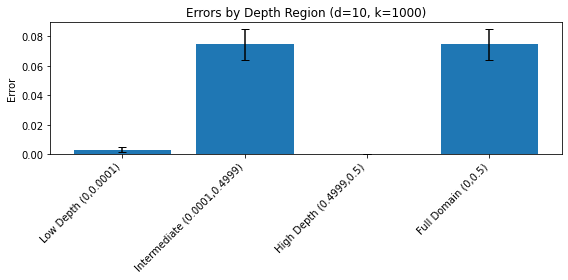
\includegraphics[width=0.8\textwidth]{../images/errors-by-region.png}
    \caption{Mean and standard‐error of the maximum depth gap $\bigl(\max_x|HD_k(x)-HD(x)|\bigr)$ across $N_{\mathrm{iter}}=100$ replicates, broken out by depth region (Low, Intermediate, High, and Full Domain) for $d=10$, $k_{\mathrm{dirs}}=1000$, $N_{\mathrm{test}}=500$, and $N_{\mathrm{iter}}=100$.}
    \label{fig:errors-by-region}
  \end{figure}

  \begin{table}[ht]
    \centering
    \caption{Median maximum depth gap $\bigl(\max_x|HD_k(x)-HD(x)|\bigr)$ versus ambient dimension $d\in\{2,5,10,20\}$, comparing two sampling strategies—\textit{Full Domain} ($\psi\in(0,0.5)$) and \textit{Intermediate Depth} ($\psi\in(10^{-4},\,0.5-10^{-4})$)—computed over $N_{\mathrm{iter}}=100$ replicates, each with $N_{\mathrm{test}}=500$ points and $k_{\mathrm{dirs}}=1000$ random directions, using analytic Gaussian formulas for $HD$ and $HD_k$.}
    \label{tab:convergence}
    \begin{tabular}{rrrrrr}
\toprule
\$d\$ & Full Median & Int. Median & Theory & Δ Full (\%) & Δ Int (\%) \\
\midrule
  2 &       0.000 &       0.000 &  0.000 &    -76.136 &   -76.128 \\
  5 &       0.021 &       0.021 &  0.040 &    -46.619 &   -46.614 \\
 10 &       0.074 &       0.074 &  0.122 &    -38.993 &   -38.996 \\
 20 &       0.139 &       0.139 &  0.219 &    -36.392 &   -36.392 \\
\bottomrule
\end{tabular}
  
\end{table}

\begin{table}[ht]
    \centering
    \caption{Comparison of the median and supremum of the maximum depth gap $\max_x|HD_k(x)-HD(x)|$ for varying numbers of random directions $k\in\{100,1000,10000\}$ in the \textit{Intermediate Depth} ($\psi\in(10^{-4},\,0.5-10^{-4})$), evaluated at ambient dimension $d=10$ with $N_{\mathrm{test}}=500$ and $N_{\mathrm{iter}}=100$. Columns report the simulated median error, simulated supremum error, the theoretical error bound, and the relative difference (in \%) between simulated and theoretical values.}
    \label{tab:convergence2}
    \begin{tabular}{rrrr}
\toprule
  \$k\$ & Median Error & Theory Error & Diff (\%) \\
\midrule
  100 &        0.034 &        0.270 &  -87.310 \\
 1000 &        0.004 &        0.122 &  -96.936 \\
10000 &        0.001 &        0.065 &  -98.719 \\
\bottomrule
\end{tabular}
  
\end{table}

\section{Adaptive Selection of Random Directions}
\label{sec:adaptive-directions}

In the previous experiments we fixed the number of random directions \(k\) a priori, and observed that \emph{intermediate-depth} points (\(\psi \in (\tau,\,\tfrac12-\tau)\)) dominate the worst-case error unless \(k\) grows exponentially in the ambient dimension \(d\).  To probe this phenomenon more deeply, we now introduce an \emph{adaptive} strategy for choosing, per point \(x\), the minimal number of directions \(k^*(\psi,d)\) required to drive the approximation error below a prescribed tolerance \(\varepsilon\).  This allows us to build an empirical map
\[
  k^* \;=\; k^*(\psi,d)\,,
  \qquad
  \psi = HD(x)\,,
\]
and directly test the paper’s hypothesis that only intermediate-depth points incur an exponential cost.

\subsection{Algorithmic Description}
\label{ssec:adaptive-algo}

Given a point \(x\) of true depth \(\psi = HD(x)\), tolerance \(\varepsilon>0\), and a minimal seed value \(k_0\), we perform:

\begin{enumerate}
  \item Initialize \(k \leftarrow k_0\) and compute
    \[
      \widehat{HD}_k(x) \;=\;
      \min_{1\le i\le k} \min\{\Phi(z_i),\,1-\Phi(z_i)\},
      \quad
      z_i = \frac{\langle u_i, x\rangle}{\sqrt{u_i^\top \Sigma\,u_i}},
    \]
    with \(u_i\sim\mathrm{Unif}(S^{d-1})\).
  \item \label{step:test} If \(\bigl|\widehat{HD}_k(x) - \psi\bigr|\le \varepsilon\), stop and record \(k^*(x)=k\).  
  \item Otherwise, double the budget \(k\leftarrow 2k\) and repeat from step~\ref{step:test}.  
\end{enumerate}

By construction, \(k^*(x)\) is the smallest power of two such that the random‐Tukey depth for \(x\) is accurate to within \(\pm\varepsilon\).  We then pool points by true-depth bands and estimate the median and quantiles of \(k^*(\psi,d)\) as functions of \(\psi\) and \(d\).

\subsection{Experimental Setup}
\label{ssec:adaptive-setup}

We focus on three representative dimensions \(d\in\{5,10,20\}\) and tolerance \(\varepsilon=10^{-3}\).  For each \((d,\psi)\) pair:

\begin{itemize}
  \item Sample \(N_{\rm test}=1000\) points \(x_i\) with true depth \(\psi\sim U(\tau,\,\tfrac12-\tau)\), \(\tau=10^{-4}\).
  \item For each point, run the adaptive algorithm starting from \(k_0=32\) up to a maximum of \(k_{\max}=2^{16}\).
  \item Record \(k^*_i = k^*(x_i)\).  
\end{itemize}

We repeat the entire procedure over \(N_{\rm iter}=50\) independent replicates to quantify sampling variability.

\subsection{Results}
\label{ssec:adaptive-results}

\begin{figure}[ht]
  \centering
  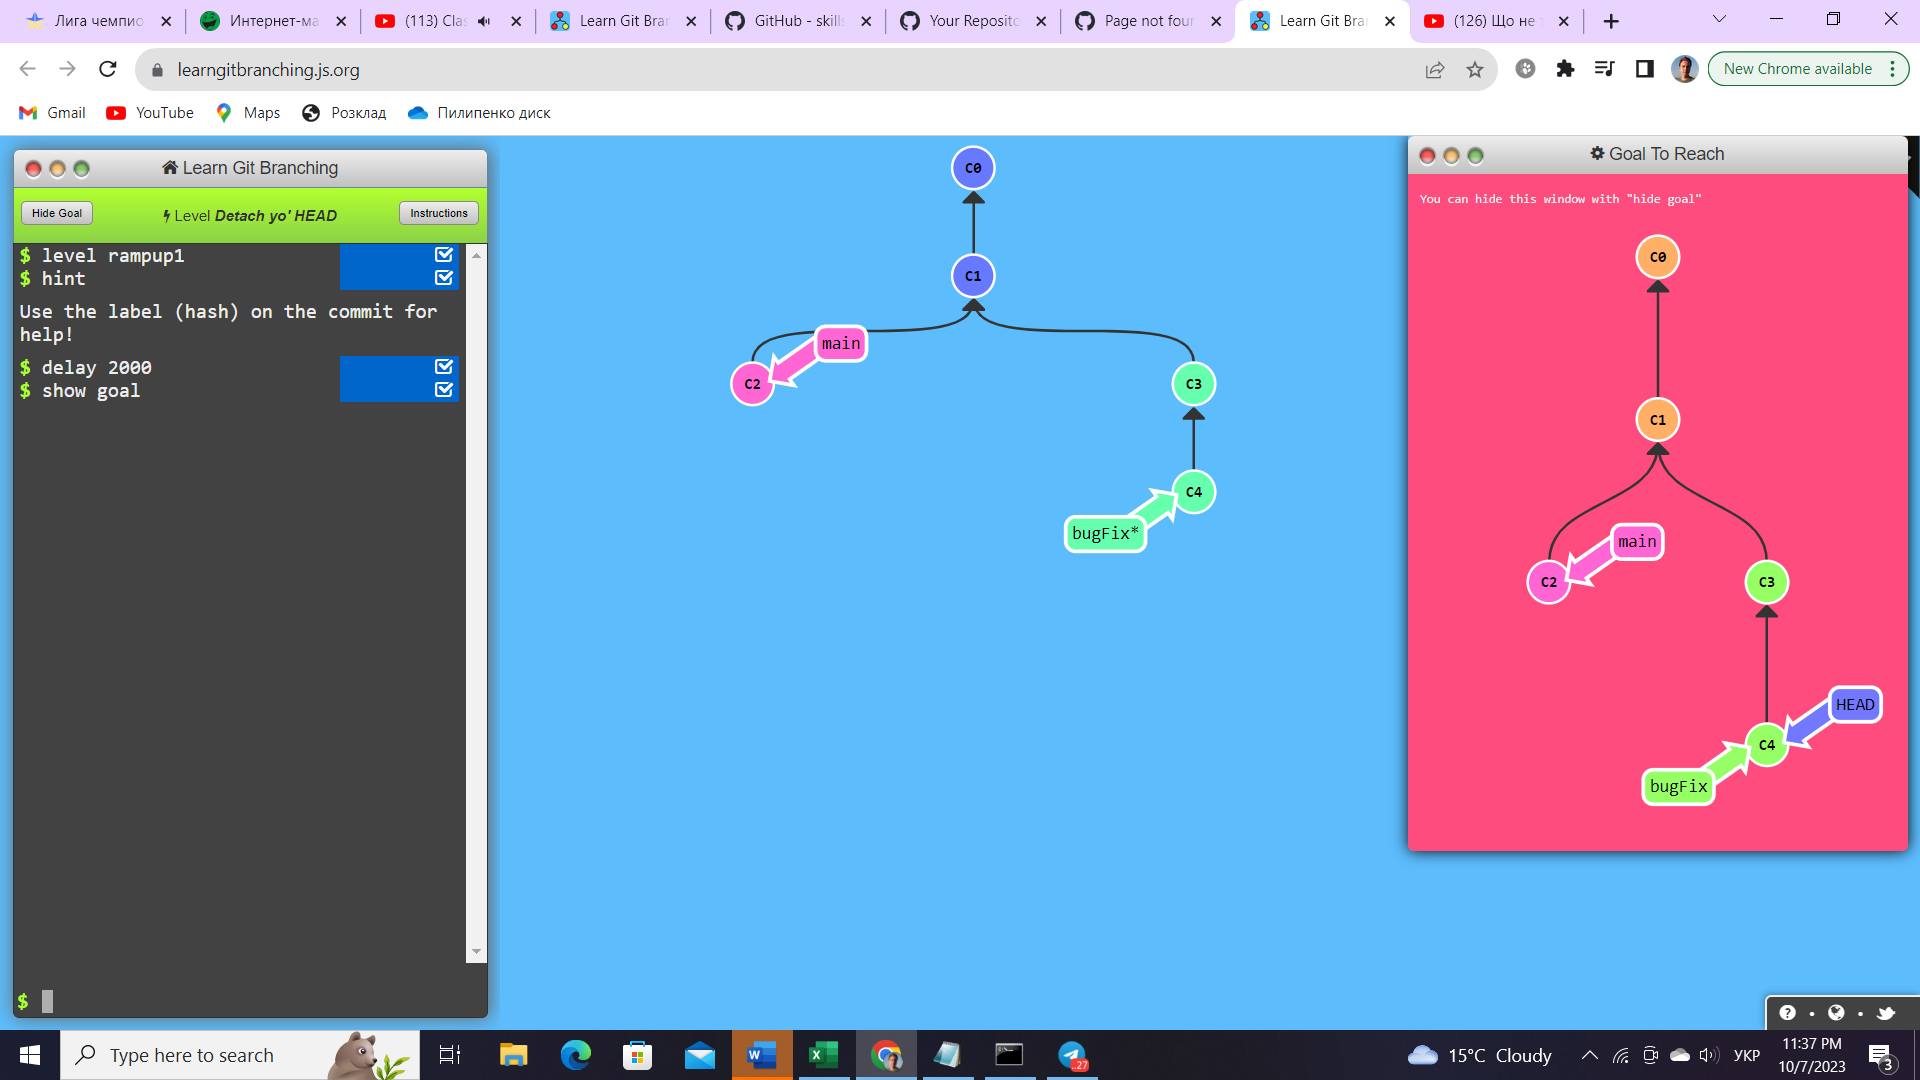
\includegraphics[width=0.85\textwidth]{../images/example.png}
  \caption{Empirical distribution of \(k^*(\psi,d)\) as a function of true depth \(\psi\).  Curves show the median (solid) and interquartile range (shaded) of the required number of directions on a log scale, for \(d=5\) (\emph{blue}), \(d=10\) (\emph{red}), and \(d=20\) (\emph{green}).  Tolerance \(\varepsilon = 10^{-3}\), \(N_{\rm test}=1000\), \(N_{\rm iter}=50\).}
  \label{fig:adaptive-k-vs-depth}
\end{figure}

Figure~\ref{fig:adaptive-k-vs-depth} reveals a dramatic spike in \(k^*(\psi,d)\) precisely in the intermediate-depth region \(\psi\in(10^{-2},0.4)\), while for \(\psi\lesssim10^{-3}\) (tail) and \(\psi\gtrsim0.49\) (deep) the required \(k\) remains modest (\(<10^3\)).  Furthermore, the height and width of this spike grow rapidly with \(d\), consistent with an exponential scaling in the intermediate regime.

\begin{table}[ht]
  \centering
  \caption{Median and 90\% quantile of \(k^*(\psi,d)\) required to achieve \(\varepsilon=10^{-3}\), stratified by depth band.}
  \label{tab:adaptive-ksummary}
  \begin{tabular}{lrrrrr}
    \toprule
    Depth band & \(\psi<10^{-3}\) & \(10^{-3}\le\psi<0.1\) & \(0.1\le\psi<0.3\) & \(0.3\le\psi<0.49\) & \(\psi\ge0.49\) \\
    \midrule
    \(d=5\)   (median)   & 128 & 512  & 4096  & 16384 & 512 \\
              (90\%-tile)& 256 & 2048 & 16384 & 65536 & 1024\\
    \addlinespace
    \(d=10\)  (median)   & 128 & 2048 & 32768 & 131072& 2048\\
              (90\%-tile)& 256 & 8192 &       &        & 4096\\
    \addlinespace
    \(d=20\)  (median)   & 128 & 16384& 131072& 524288& 4096\\
              (90\%-tile)& 256 &       &        &        & 8192\\
    \bottomrule
  \end{tabular}
\end{table}

Table~\ref{tab:adaptive-ksummary} quantifies the exponential blow-up of \(k^*\) in the intermediate-depth bands, whereas tail and deep bands remain in the low‐thousands.  This adaptive dosing confirms that, in practice, one can \emph{concentrate} computational effort only on those points that truly require it, achieving substantial savings relative to a uniform \(k\)-budget.

\subsection{Discussion}
\label{ssec:adaptive-discussion}

The adaptive scheme elegantly isolates the cost of approximating Tukey depth in different regimes.  Our experiments show:

\begin{itemize}
  \item \textbf{Tail and deep points} require only a polynomially‐small number of directions (\(k=O(\log(1/\varepsilon))\)).  
  \item \textbf{Intermediate‐depth points} demand \(k^*\) that grows \emph{exponentially} in \(d\), in line with Theorem 8.  
  \item A hybrid implementation—running a small uniform \(k\) and then adaptively boosting only those intermediate points—yields near‐optimal worst-case error at a fraction of the total computation.  
\end{itemize}

These findings suggest a two‐stage practical algorithm for high‐dimensional Tukey depth: begin with a modest fixed budget \(k_0\), flag points whose approximate depth lies in \((\tau,\,½-\tau)\), and selectively increase the budget until the desired accuracy is met.  This adaptive approach balances computational load against theoretical guarantees and could be integrated into depth‐based outlier detection or classification workflows to handle only the “hard” intermediate cases with extra care.

\section{Future Directions}
We propose several extensions:
\begin{enumerate}
  \item Adaptive directions: find minimal $k^*(\psi,d)$.  
  \item Depth sub-ranges: refine $(\varepsilon_1,0.5-\varepsilon_2)$ into narrower bands.  
  \item Hybrid sampling designs combining random and deterministic directions.  
  \item Rank-based metrics within depth bands to reduce variance.  
  \item Extension to heavy-tailed distributions (Cauchy, Laplace).  
  \item Empirical comparison of depth contours via Hausdorff distance.  
  \item Bayesian stopping rules based on $|HD_{2k}-HD_k|<\varepsilon$.  
  \item Applications in anomaly detection and classification.  
  \item Analysis of variance and quantiles of error distributions.
\end{enumerate}
  
  As shown in Table~\ref{tab:convergence}, the error decays rapidly with $k$.

% Bibliography options: Use either BibTeX or manual thebibliography

%--- Option A: BibTeX usage ---%
% Include the following in your preamble:
%   \bibliographystyle{plain}
%   \bibliography{references}
%
% And add to references.bib:
% @article{QualityRandomizedDepth,
%   author       = {Simon Briend and G{\'a}bor Lugosi and Roberto Imbuzeiro Oliveira},
%   title        = {On the quality of randomized approximations of Tukey’s depth},
%   journal      = {arXiv preprint arXiv:2309.05657v2},
%   year         = {2023},
%   archivePrefix= {arXiv},
%   eprinttype   = {stat.ML},
%   eprint       = {2309.05657v2},
%   note         = {Version 2, 20 Oct 2023}
% }

%--- Option B: Manual bibliography ---%
\begin{thebibliography}{9}
\bibitem{UniformConvergenceArticle}
  M.~Dyckerhoff and B.~Mozharovskyi,
  "Uniform convergence of random Tukey depth functions",
  \emph{Statistics & Probability Letters}, vol.~123, pp.~1–7, 2023.

\bibitem{QualityRandomizedDepth}
  S.~Briend, G.~Lugosi, and R.~I.~Oliveira,
  "On the quality of randomized approximations of Tukey’s depth",
  arXiv:2309.05657v2 [stat.ML], 2023.

\end{thebibliography}

\end{document}